% Graphic for TeX using PGF
% Title: /home/satenske/cours/AP/obj3/uml3dia
% Creator: Dia v0.97.1
% CreationDate: Thu Sep 15 10:23:25 2011
% For: satenske
% \usepackage{tikz}
% The following commands are not supported in PSTricks at present
% We define them conditionally, so when they are implemented,
% this pgf file will use them.
\ifx\du\undefined
  \newlength{\du}
\fi
\setlength{\du}{15\unitlength}
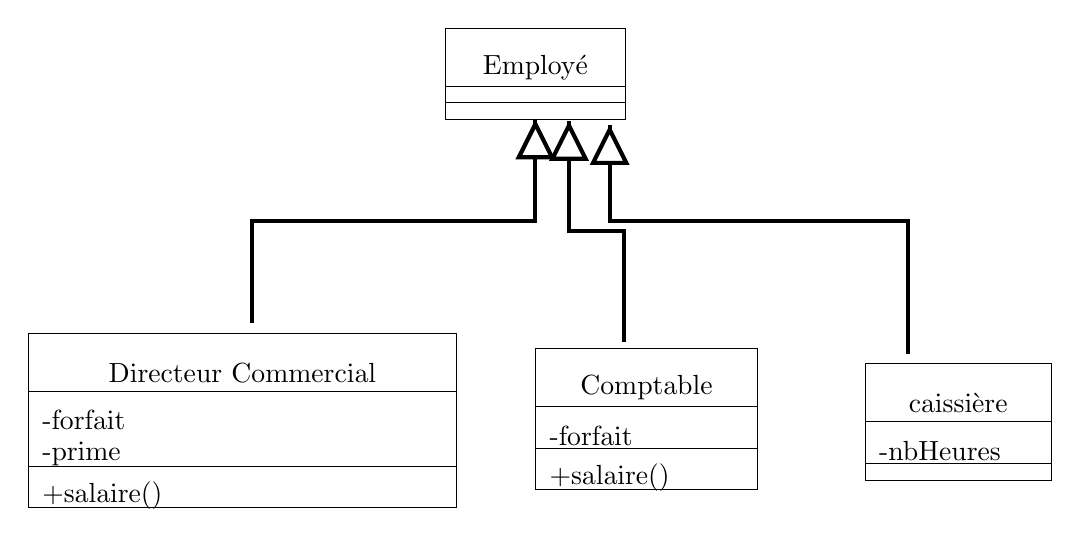
\begin{tikzpicture}
\pgftransformxscale{1.000000}
\pgftransformyscale{-1.000000}
\definecolor{dialinecolor}{rgb}{0.000000, 0.000000, 0.000000}
\pgfsetstrokecolor{dialinecolor}
\definecolor{dialinecolor}{rgb}{1.000000, 1.000000, 1.000000}
\pgfsetfillcolor{dialinecolor}
\pgfsetlinewidth{0.020000\du}
\pgfsetdash{}{0pt}
\definecolor{dialinecolor}{rgb}{1.000000, 1.000000, 1.000000}
\pgfsetfillcolor{dialinecolor}
\fill (10.700000\du,2.950000\du)--(10.700000\du,4.350000\du)--(15.042500\du,4.350000\du)--(15.042500\du,2.950000\du)--cycle;
\definecolor{dialinecolor}{rgb}{0.000000, 0.000000, 0.000000}
\pgfsetstrokecolor{dialinecolor}
\draw (10.700000\du,2.950000\du)--(10.700000\du,4.350000\du)--(15.042500\du,4.350000\du)--(15.042500\du,2.950000\du)--cycle;
% setfont left to latex
\definecolor{dialinecolor}{rgb}{0.000000, 0.000000, 0.000000}
\pgfsetstrokecolor{dialinecolor}
\node at (12.871250\du,3.900000\du){Employé};
\definecolor{dialinecolor}{rgb}{1.000000, 1.000000, 1.000000}
\pgfsetfillcolor{dialinecolor}
\fill (10.700000\du,4.350000\du)--(10.700000\du,4.750000\du)--(15.042500\du,4.750000\du)--(15.042500\du,4.350000\du)--cycle;
\definecolor{dialinecolor}{rgb}{0.000000, 0.000000, 0.000000}
\pgfsetstrokecolor{dialinecolor}
\draw (10.700000\du,4.350000\du)--(10.700000\du,4.750000\du)--(15.042500\du,4.750000\du)--(15.042500\du,4.350000\du)--cycle;
\definecolor{dialinecolor}{rgb}{1.000000, 1.000000, 1.000000}
\pgfsetfillcolor{dialinecolor}
\fill (10.700000\du,4.750000\du)--(10.700000\du,5.150000\du)--(15.042500\du,5.150000\du)--(15.042500\du,4.750000\du)--cycle;
\definecolor{dialinecolor}{rgb}{0.000000, 0.000000, 0.000000}
\pgfsetstrokecolor{dialinecolor}
\draw (10.700000\du,4.750000\du)--(10.700000\du,5.150000\du)--(15.042500\du,5.150000\du)--(15.042500\du,4.750000\du)--cycle;
\pgfsetlinewidth{0.020000\du}
\pgfsetdash{}{0pt}
\definecolor{dialinecolor}{rgb}{1.000000, 1.000000, 1.000000}
\pgfsetfillcolor{dialinecolor}
\fill (0.650000\du,10.300000\du)--(0.650000\du,11.700000\du)--(10.975000\du,11.700000\du)--(10.975000\du,10.300000\du)--cycle;
\definecolor{dialinecolor}{rgb}{0.000000, 0.000000, 0.000000}
\pgfsetstrokecolor{dialinecolor}
\draw (0.650000\du,10.300000\du)--(0.650000\du,11.700000\du)--(10.975000\du,11.700000\du)--(10.975000\du,10.300000\du)--cycle;
% setfont left to latex
\definecolor{dialinecolor}{rgb}{0.000000, 0.000000, 0.000000}
\pgfsetstrokecolor{dialinecolor}
\node at (5.812500\du,11.250000\du){Directeur Commercial};
\definecolor{dialinecolor}{rgb}{1.000000, 1.000000, 1.000000}
\pgfsetfillcolor{dialinecolor}
\fill (0.650000\du,11.700000\du)--(0.650000\du,13.500000\du)--(10.975000\du,13.500000\du)--(10.975000\du,11.700000\du)--cycle;
\definecolor{dialinecolor}{rgb}{0.000000, 0.000000, 0.000000}
\pgfsetstrokecolor{dialinecolor}
\draw (0.650000\du,11.700000\du)--(0.650000\du,13.500000\du)--(10.975000\du,13.500000\du)--(10.975000\du,11.700000\du)--cycle;
% setfont left to latex
\definecolor{dialinecolor}{rgb}{0.000000, 0.000000, 0.000000}
\pgfsetstrokecolor{dialinecolor}
\node[anchor=west] at (0.760000\du,12.400000\du){-forfait};
% setfont left to latex
\definecolor{dialinecolor}{rgb}{0.000000, 0.000000, 0.000000}
\pgfsetstrokecolor{dialinecolor}
\node[anchor=west] at (0.760000\du,13.200000\du){-prime};
\definecolor{dialinecolor}{rgb}{1.000000, 1.000000, 1.000000}
\pgfsetfillcolor{dialinecolor}
\fill (0.650000\du,13.500000\du)--(0.650000\du,14.500000\du)--(10.975000\du,14.500000\du)--(10.975000\du,13.500000\du)--cycle;
\definecolor{dialinecolor}{rgb}{0.000000, 0.000000, 0.000000}
\pgfsetstrokecolor{dialinecolor}
\draw (0.650000\du,13.500000\du)--(0.650000\du,14.500000\du)--(10.975000\du,14.500000\du)--(10.975000\du,13.500000\du)--cycle;
% setfont left to latex
\definecolor{dialinecolor}{rgb}{0.000000, 0.000000, 0.000000}
\pgfsetstrokecolor{dialinecolor}
\node[anchor=west] at (0.760000\du,14.200000\du){+salaire()};
\pgfsetlinewidth{0.020000\du}
\pgfsetdash{}{0pt}
\definecolor{dialinecolor}{rgb}{1.000000, 1.000000, 1.000000}
\pgfsetfillcolor{dialinecolor}
\fill (20.810000\du,11.035000\du)--(20.810000\du,12.435000\du)--(25.305000\du,12.435000\du)--(25.305000\du,11.035000\du)--cycle;
\definecolor{dialinecolor}{rgb}{0.000000, 0.000000, 0.000000}
\pgfsetstrokecolor{dialinecolor}
\draw (20.810000\du,11.035000\du)--(20.810000\du,12.435000\du)--(25.305000\du,12.435000\du)--(25.305000\du,11.035000\du)--cycle;
% setfont left to latex
\definecolor{dialinecolor}{rgb}{0.000000, 0.000000, 0.000000}
\pgfsetstrokecolor{dialinecolor}
\node at (23.057500\du,11.985000\du){caissière};
\definecolor{dialinecolor}{rgb}{1.000000, 1.000000, 1.000000}
\pgfsetfillcolor{dialinecolor}
\fill (20.810000\du,12.435000\du)--(20.810000\du,13.435000\du)--(25.305000\du,13.435000\du)--(25.305000\du,12.435000\du)--cycle;
\definecolor{dialinecolor}{rgb}{0.000000, 0.000000, 0.000000}
\pgfsetstrokecolor{dialinecolor}
\draw (20.810000\du,12.435000\du)--(20.810000\du,13.435000\du)--(25.305000\du,13.435000\du)--(25.305000\du,12.435000\du)--cycle;
% setfont left to latex
\definecolor{dialinecolor}{rgb}{0.000000, 0.000000, 0.000000}
\pgfsetstrokecolor{dialinecolor}
\node[anchor=west] at (20.920000\du,13.135000\du){-nbHeures};
\definecolor{dialinecolor}{rgb}{1.000000, 1.000000, 1.000000}
\pgfsetfillcolor{dialinecolor}
\fill (20.810000\du,13.435000\du)--(20.810000\du,13.835000\du)--(25.305000\du,13.835000\du)--(25.305000\du,13.435000\du)--cycle;
\definecolor{dialinecolor}{rgb}{0.000000, 0.000000, 0.000000}
\pgfsetstrokecolor{dialinecolor}
\draw (20.810000\du,13.435000\du)--(20.810000\du,13.835000\du)--(25.305000\du,13.835000\du)--(25.305000\du,13.435000\du)--cycle;
\pgfsetlinewidth{0.020000\du}
\pgfsetdash{}{0pt}
\definecolor{dialinecolor}{rgb}{1.000000, 1.000000, 1.000000}
\pgfsetfillcolor{dialinecolor}
\fill (12.870000\du,10.670000\du)--(12.870000\du,12.070000\du)--(18.225000\du,12.070000\du)--(18.225000\du,10.670000\du)--cycle;
\definecolor{dialinecolor}{rgb}{0.000000, 0.000000, 0.000000}
\pgfsetstrokecolor{dialinecolor}
\draw (12.870000\du,10.670000\du)--(12.870000\du,12.070000\du)--(18.225000\du,12.070000\du)--(18.225000\du,10.670000\du)--cycle;
% setfont left to latex
\definecolor{dialinecolor}{rgb}{0.000000, 0.000000, 0.000000}
\pgfsetstrokecolor{dialinecolor}
\node at (15.547500\du,11.620000\du){Comptable};
\definecolor{dialinecolor}{rgb}{1.000000, 1.000000, 1.000000}
\pgfsetfillcolor{dialinecolor}
\fill (12.870000\du,12.070000\du)--(12.870000\du,13.070000\du)--(18.225000\du,13.070000\du)--(18.225000\du,12.070000\du)--cycle;
\definecolor{dialinecolor}{rgb}{0.000000, 0.000000, 0.000000}
\pgfsetstrokecolor{dialinecolor}
\draw (12.870000\du,12.070000\du)--(12.870000\du,13.070000\du)--(18.225000\du,13.070000\du)--(18.225000\du,12.070000\du)--cycle;
% setfont left to latex
\definecolor{dialinecolor}{rgb}{0.000000, 0.000000, 0.000000}
\pgfsetstrokecolor{dialinecolor}
\node[anchor=west] at (12.980000\du,12.770000\du){-forfait};
\definecolor{dialinecolor}{rgb}{1.000000, 1.000000, 1.000000}
\pgfsetfillcolor{dialinecolor}
\fill (12.870000\du,13.070000\du)--(12.870000\du,14.070000\du)--(18.225000\du,14.070000\du)--(18.225000\du,13.070000\du)--cycle;
\definecolor{dialinecolor}{rgb}{0.000000, 0.000000, 0.000000}
\pgfsetstrokecolor{dialinecolor}
\draw (12.870000\du,13.070000\du)--(12.870000\du,14.070000\du)--(18.225000\du,14.070000\du)--(18.225000\du,13.070000\du)--cycle;
% setfont left to latex
\definecolor{dialinecolor}{rgb}{0.000000, 0.000000, 0.000000}
\pgfsetstrokecolor{dialinecolor}
\node[anchor=west] at (12.980000\du,13.770000\du){+salaire()};
\pgfsetlinewidth{0.100000\du}
\pgfsetdash{}{0pt}
\pgfsetmiterjoin
\pgfsetbuttcap
{
\definecolor{dialinecolor}{rgb}{0.000000, 0.000000, 0.000000}
\pgfsetfillcolor{dialinecolor}
% was here!!!
\definecolor{dialinecolor}{rgb}{0.000000, 0.000000, 0.000000}
\pgfsetstrokecolor{dialinecolor}
\draw (12.871250\du,5.150000\du)--(12.871250\du,7.600000\du)--(6.050000\du,7.600000\du)--(6.050000\du,10.050000\du);
}
\definecolor{dialinecolor}{rgb}{0.000000, 0.000000, 0.000000}
\pgfsetstrokecolor{dialinecolor}
\draw (12.871250\du,6.061803\du)--(12.871250\du,7.600000\du)--(6.050000\du,7.600000\du)--(6.050000\du,10.050000\du);
\pgfsetmiterjoin
\definecolor{dialinecolor}{rgb}{1.000000, 1.000000, 1.000000}
\pgfsetfillcolor{dialinecolor}
\fill (13.271250\du,6.061803\du)--(12.871250\du,5.261803\du)--(12.471250\du,6.061803\du)--cycle;
\pgfsetlinewidth{0.100000\du}
\pgfsetdash{}{0pt}
\pgfsetmiterjoin
\definecolor{dialinecolor}{rgb}{0.000000, 0.000000, 0.000000}
\pgfsetstrokecolor{dialinecolor}
\draw (13.271250\du,6.061803\du)--(12.871250\du,5.261803\du)--(12.471250\du,6.061803\du)--cycle;
% setfont left to latex
\pgfsetlinewidth{0.100000\du}
\pgfsetdash{}{0pt}
\pgfsetmiterjoin
\pgfsetbuttcap
{
\definecolor{dialinecolor}{rgb}{0.000000, 0.000000, 0.000000}
\pgfsetfillcolor{dialinecolor}
% was here!!!
\definecolor{dialinecolor}{rgb}{0.000000, 0.000000, 0.000000}
\pgfsetstrokecolor{dialinecolor}
\draw (13.681250\du,5.185000\du)--(13.681250\du,7.842500\du)--(15.000000\du,7.842500\du)--(15.000000\du,10.500000\du);
}
\definecolor{dialinecolor}{rgb}{0.000000, 0.000000, 0.000000}
\pgfsetstrokecolor{dialinecolor}
\draw (13.681250\du,6.096803\du)--(13.681250\du,7.842500\du)--(15.000000\du,7.842500\du)--(15.000000\du,10.500000\du);
\pgfsetmiterjoin
\definecolor{dialinecolor}{rgb}{1.000000, 1.000000, 1.000000}
\pgfsetfillcolor{dialinecolor}
\fill (14.081250\du,6.096803\du)--(13.681250\du,5.296803\du)--(13.281250\du,6.096803\du)--cycle;
\pgfsetlinewidth{0.100000\du}
\pgfsetdash{}{0pt}
\pgfsetmiterjoin
\definecolor{dialinecolor}{rgb}{0.000000, 0.000000, 0.000000}
\pgfsetstrokecolor{dialinecolor}
\draw (14.081250\du,6.096803\du)--(13.681250\du,5.296803\du)--(13.281250\du,6.096803\du)--cycle;
% setfont left to latex
\pgfsetlinewidth{0.100000\du}
\pgfsetdash{}{0pt}
\pgfsetmiterjoin
\pgfsetbuttcap
{
\definecolor{dialinecolor}{rgb}{0.000000, 0.000000, 0.000000}
\pgfsetfillcolor{dialinecolor}
% was here!!!
\definecolor{dialinecolor}{rgb}{0.000000, 0.000000, 0.000000}
\pgfsetstrokecolor{dialinecolor}
\draw (14.660000\du,5.285000\du)--(14.660000\du,7.600000\du)--(21.850000\du,7.600000\du)--(21.850000\du,10.800000\du);
}
\definecolor{dialinecolor}{rgb}{0.000000, 0.000000, 0.000000}
\pgfsetstrokecolor{dialinecolor}
\draw (14.660000\du,6.196803\du)--(14.660000\du,7.600000\du)--(21.850000\du,7.600000\du)--(21.850000\du,10.800000\du);
\pgfsetmiterjoin
\definecolor{dialinecolor}{rgb}{1.000000, 1.000000, 1.000000}
\pgfsetfillcolor{dialinecolor}
\fill (15.060000\du,6.196803\du)--(14.660000\du,5.396803\du)--(14.260000\du,6.196803\du)--cycle;
\pgfsetlinewidth{0.100000\du}
\pgfsetdash{}{0pt}
\pgfsetmiterjoin
\definecolor{dialinecolor}{rgb}{0.000000, 0.000000, 0.000000}
\pgfsetstrokecolor{dialinecolor}
\draw (15.060000\du,6.196803\du)--(14.660000\du,5.396803\du)--(14.260000\du,6.196803\du)--cycle;
% setfont left to latex
\end{tikzpicture}
